\section{ProtoDUNE-ND detector physics studies}
\label{sec:detector-physics-studies}
Basic detector stability checks will be checked with a period of detector operation in Bern before moving the module to Fermilab. These tests would include extraction and re-insertion tests of individual modules into the LAr bath, and checks that the LAr purity is sufficient. However, local tests can only be performed using cosmic muons, which have limited utility beyond basic detector stability checks. In this section, we identify a number of key detector physics questions which could be answered by the ProtoDUNE-ND test, and would help inform the final design of the full ArgonCube ND component for DUNE, and aid in developing reconstruction algorithms suitable for neutrino interactions.

In order to check the feasibility of these studies, two different simulations were used. Firstly, high statistics GENIE \todo{and NEUT?} Monte Carlo samples were produced, in order to compare basic properties of neutrino interactions expected in the LBNF and NuMI ME beamlines. Secondly, GENIE events were used to seed a basic GEANT4 simulation, using the ArgonBox software, in order to get a basic understanding of event shape and containment. In the latter simulation, events were simulated in an infinite box of LAr, and were then distributed randomly inside a volume with the correct spatial dimensions as the 2x2 demonstrator module. Although the 2x2 geometry was not included in the simulation, this gives an acceptable estimate of the expected event rates for the studies described below. \todo{Patrick/Chris to expand this clumsy description of ArgonBox. Is there a reference I should use?}. Examples of the ArgonBox simulation with the basic 2x2 geometry superimposed can be seen in Figure~\ref{} for a number of different neutrino energies.

\todo{Add a figure with Patrick's event display images for a couple of neutrino energies}

%\subsection{Track multiplicity, rate and pile-up}
\begin{figure}[htb]
  \centering
  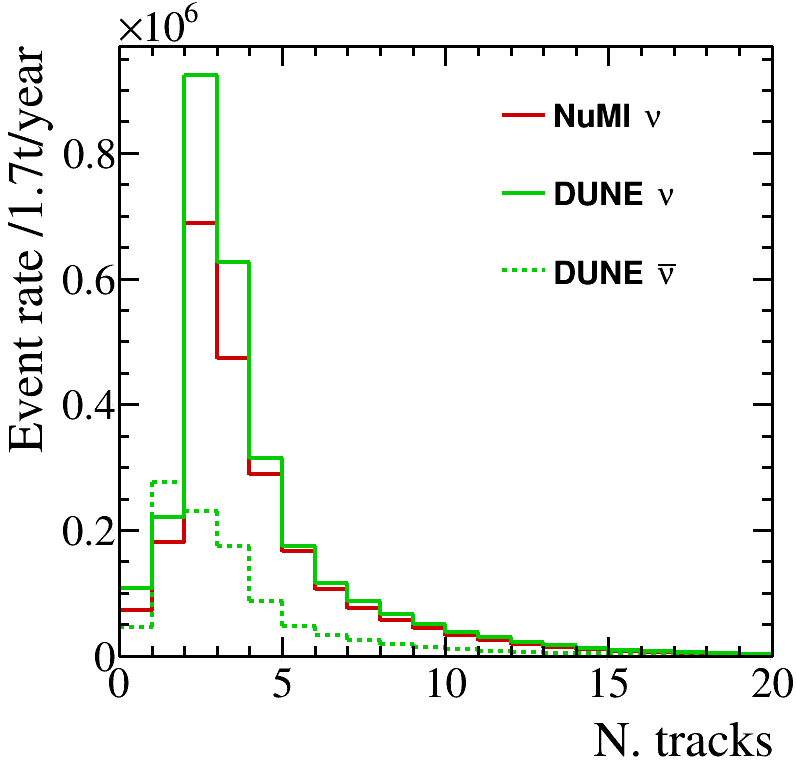
\includegraphics[width=0.5\textwidth]{plots/2x2_ntracks_all.png}
  \caption{The expected yearly rates of minimum and highly ionizing particles expected in the 2x2 module's 1.7t LAr volume for the NuMI ME and LBNF fluxes, produced using GENIE v2.12.8 with the ``ValenciaQEBergerSehgalCOHRES'' configuration~\cite{genie}.}
  \label{fig:track_multiplicity}
\end{figure}
In order to be a relevant test for the full ArgonCube near detector, which will be in the LBNF beamline, it is useful to first verify that the basic properties of the events are similar, despite the NuMI ME beam being somewhat higher energy than the planned LBNF beam (as shown in Figure~\ref{fig:beam_options}). Figure~\ref{fig:track_multiplicity} shows the expected multiplicity of minimum or highly ionizing tracks at the vertex for both the LBNF and NuMI ME beams, in neutrino and antineutrino mode, produced with the GENIE generator. The track multiplicities are similar, which indicates that the scale of the reconstruction problem is similar, and the proposed ProtoDUNE-ND test will be a useful benchmark for developing the ArgonCube reconstruction software.

\begin{figure}[htb]
  \centering
  \subfloat[$\mu^{\pm}$] {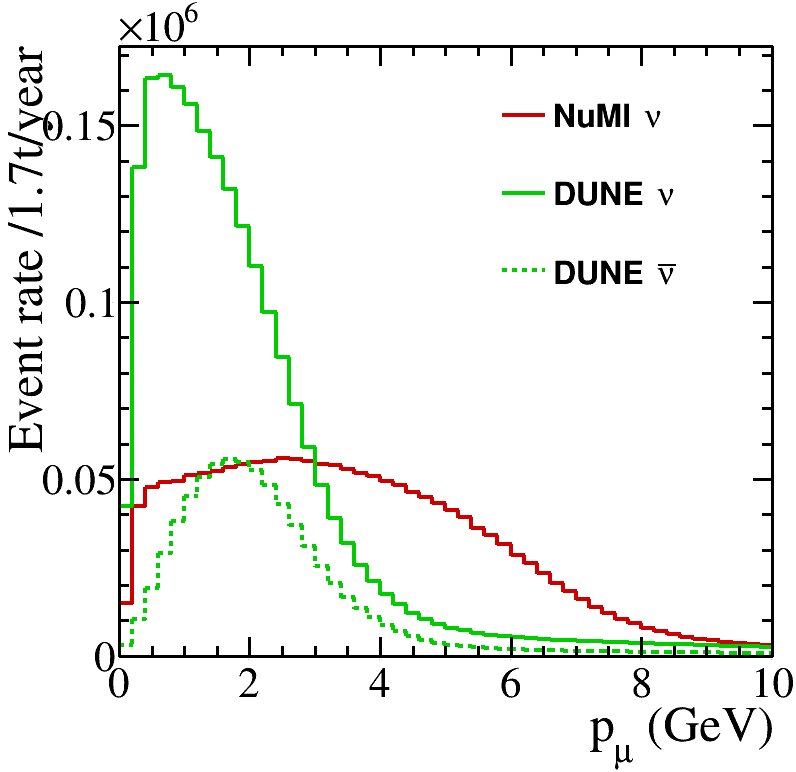
\includegraphics[width=0.5\textwidth]{plots/2x2_muon_mom_all.png}}
  \subfloat[Protons]    {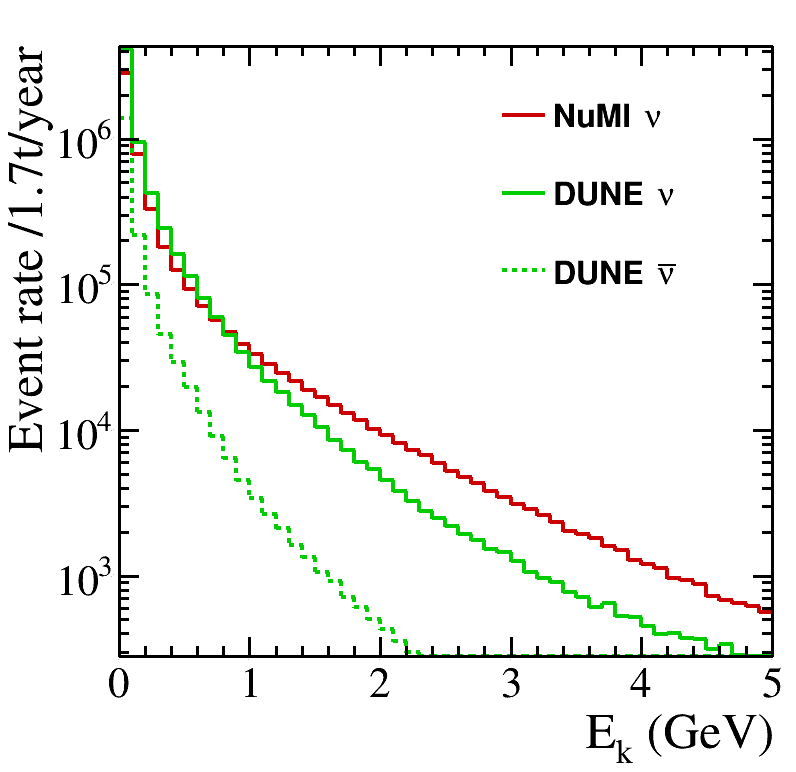
\includegraphics[width=0.5\textwidth]{plots/2x2_proton_Ek_all.png}}\\
  \subfloat[$\pi^{+}$]    {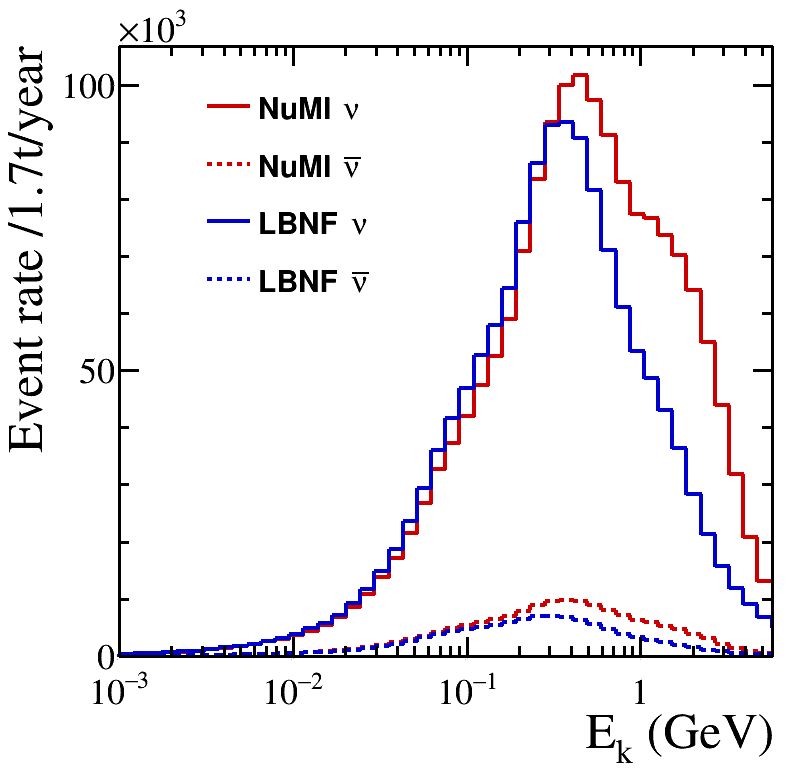
\includegraphics[width=0.5\textwidth]{plots/2x2_piplus_Ek_all.png}}
  \subfloat[$\pi^{-}$]    {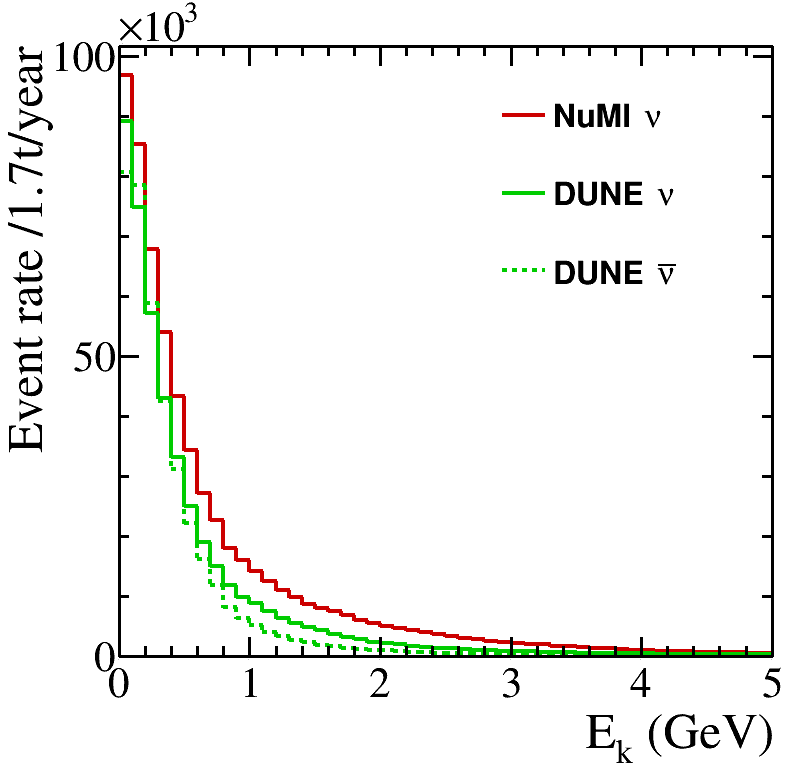
\includegraphics[width=0.5\textwidth]{plots/2x2_piminus_Ek_all.png}}  
  \caption{The expected yearly rates of various particles produced at the vertex, as a function of their kinetic energy, expected in the 2x2 module's 1.7t LAr volume for the NuMI ME and LBNF fluxes, produced using GENIE v2.12.8 with the ``ValenciaQEBergerSehgalCOHRES'' configuration~\cite{genie}. Note that every relevant particle from each event is included. \todo{Get the muon kinetic energy!}}
  \label{fig:kinetic_energies}
\end{figure}
In Figure~\ref{fig:kinetic_energies}, the kinetic energies of various particles coming from the initial neutrino--argon vertex are compared for the LBNF and NuMI ME beams. As expected, the energy distributions of all of the particles are slightly broader for the NuMI ME flux, but there are significant numbers of events with particle kinematics across the broad range of energies expected for the LBNF beams.

In the full ArgonCube detector and the more intense LBNF beamline, pile-up will be an additional challenge. \todo{Patrick to add a comment on pile-up at NuMI}. Additionally, the relatively small size of the 2x2 Demonstrator module means that relatively fewer of the tracks will be contained, making particle identification (PID) studies challenging, except for the cases listed below. Although other detectors are not included in the ArgonBox simulation, the lack of containment and PID capabilities mean that including another subdetector in the ProtoDUNE-ND setup is essential for any ancilliary physics measurements to be made.

\FloatBarrier
\subsection{Combining light and charge signals}
An important first test of the detector is how well the prompt light collection efficiency is, and how well the light readout can be combined with charge readout to reconstruct events

\subsection{Identifying neutrons}
\todo{Patrick}
\begin{figure}[htb]
  \centering
  \subfloat[Neutron multiplicity]   {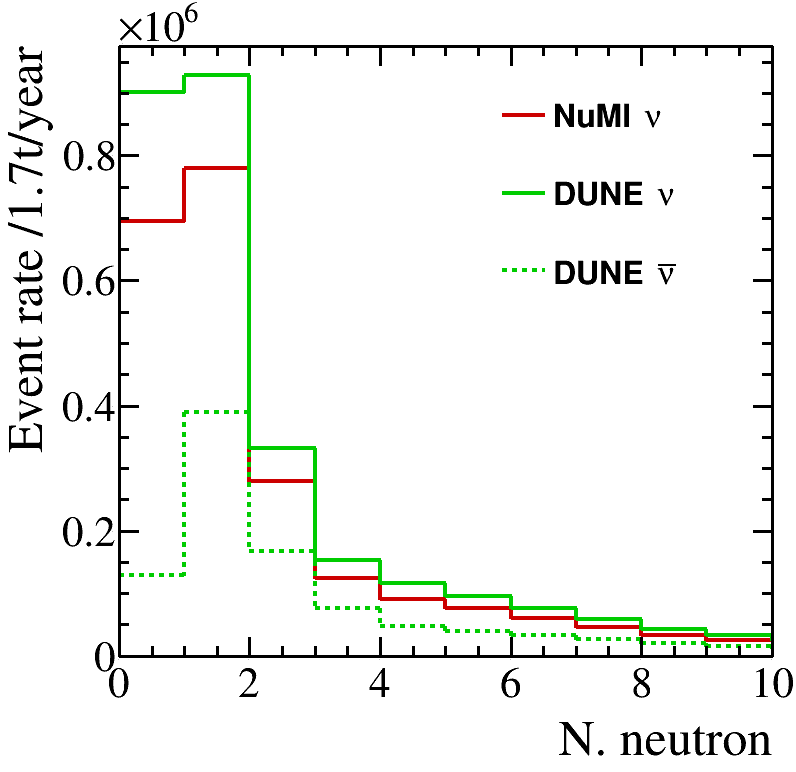
\includegraphics[width=0.5\textwidth]{plots/2x2_nneutron_all.png}}
  \subfloat[Neutron kinetic energy] {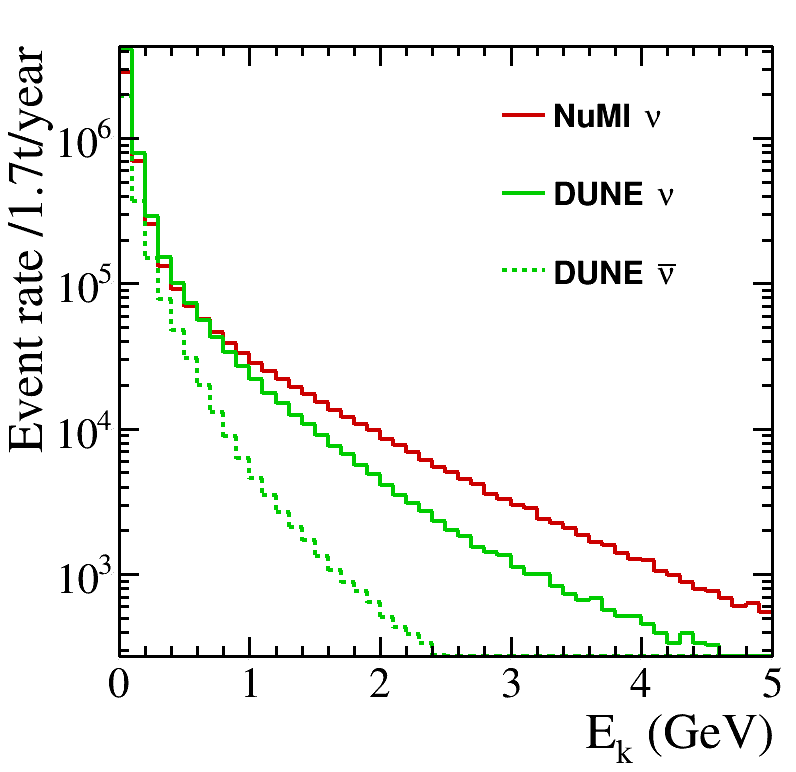
\includegraphics[width=0.5\textwidth]{plots/2x2_neutron_Ek_all.png}}  
  \caption{The expected yearly rates of $\pi^{0}$'s produced at the vertex, as a function of event multiplicity and their kinetic energy, expected in the 2x2 module's 1.7t LAr volume for the NuMI ME and LBNF fluxes, produced using GENIE v2.12.8 with the ``ValenciaQEBergerSehgalCOHRES'' configuration~\cite{genie}. Note that every $\pi^{0}$ from each event is included.}
  \label{fig:pi0_kinematics}
\end{figure}

\subsection{Cosmic suppression}
\todo{Is this worth commenting on? If we have scintillator paddles, we can find out how often the reconstruction mistakes cosmics for beam events. Should be easy with ArcLight and not being mICRObOOne, but might be worth commenting on...}. What's the nominal cosmic suppression rate? How often would we expect to see a cosmic in the 2x2 drift window?

\subsection{Track reconstruction across modules}
\todo{stole this from the LOI}  The module walls produce gaps in particle tracks traversing multiple modules similar to dead wires in classic LArTPC readouts.
Algorithms to join such segmented tracks already exist~\cite{pandora}.
However, a detailed study of the influence of module walls on reconstruction efficiency still needs to be performed.

\subsection{Shower reconstruction across modules}
Charge sharing of EM and hadronic showers between modules. Need Patrick's studies of shower depth, how many showers will be contained, how many not, etc etc

\subsection{Electron-photon separation}
Lots of pi0s, MicroBooNE can't do it well. Build's on Damian's work --> look at his thesis for this. Actually, Damian's work is a bit confusing. Surely we want to reconstruct pi0 invariant mass peaks? This could be a pretty useful measure of the lost shower energy?
\begin{figure}[htb]
  \centering
  \subfloat[$\pi^{0}$ multiplicity]   {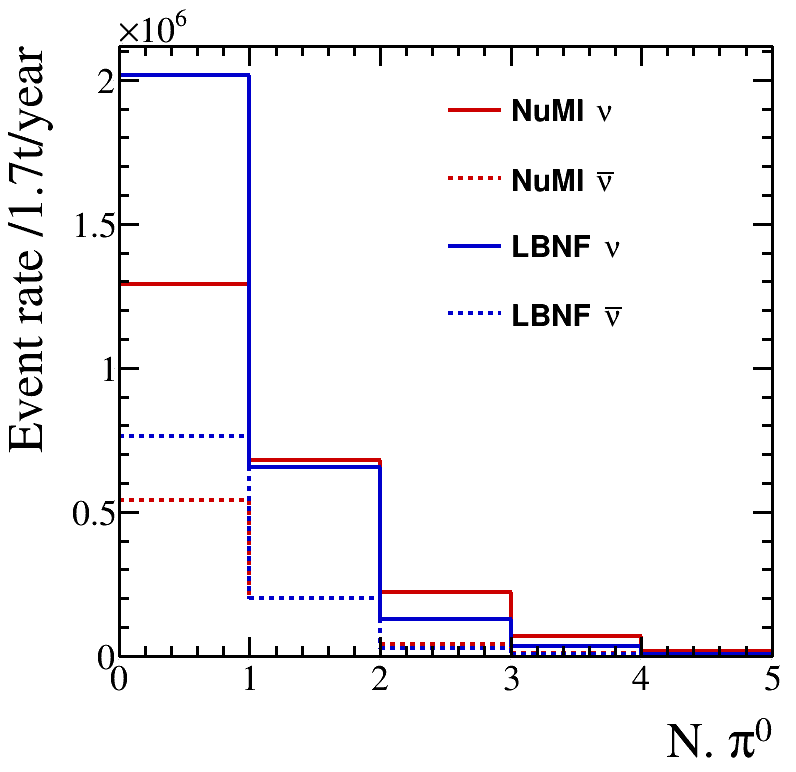
\includegraphics[width=0.5\textwidth]{plots/2x2_npi0_all.png}}
  \subfloat[$\pi^{0}$ kinetic energy] {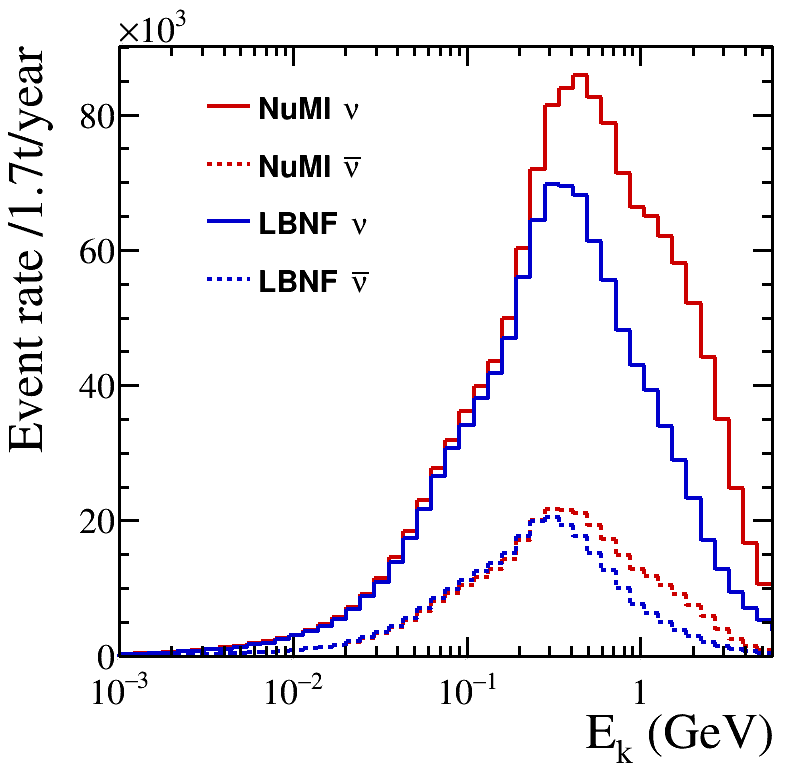
\includegraphics[width=0.5\textwidth]{plots/2x2_pi0_Ek_all.png}}  
  \caption{The expected yearly rates of $\pi^{0}$'s produced at the vertex, as a function of event multiplicity and their kinetic energy, expected in the 2x2 module's 1.7t LAr volume for the NuMI ME and LBNF fluxes, produced using GENIE v2.12.8 with the ``ValenciaQEBergerSehgalCOHRES'' configuration~\cite{genie}. Note that every $\pi^{0}$ from each event is included.}
  \label{fig:pi0_kinematics}
\end{figure}

\FloatBarrier
\subsection{Michel tagging}
\todo{Figure out if we can do anything remotely reasonable... Patrick could see how many stopped muons/pions he has. But I'm not sure how we get the efficiency from that...}

\subsection{Proton tagging}
\todo{Worth commenting on figuring out how well we can find Bragg peaks? Do we care for this test?}

\subsection{Electric field uniformity and space charge build-up}
A concern for LAr detectors in a high intensity beam is the build up of space charge --- long-lived argon ions which drift slowly towards the cathode --- and possible affects on the uniformity of the electric field which may accumulate over time. In currently operating and near-future LAr detectors~\addcite (uB and SBND), both cosmic tracks and UV lasers are used to calibrate for distortions in the electric field. Both the UV laser track and high energy cosmic muons are expected to leave straight tracks in the detector. If the drift field is not uniform across the detector, ionization electrons produced along the length of this track will not drift at the same speed, and will result in a distorted track at the readout plane. By comparing the reconstructed and expected track, a map of the electric field distortion can be built up for calibration purposes.

Assuming that the 2x2 demonstrator module is equipped with scintillator panels to tag cosmic tracks using a timing coincidence between two sides of the detector, and reasonable spatial resolution on those scintillator paddles, electric field distortions could be measured in the 2x2 demonstrator module. By looking at beam-on, and beam-off data, it would be possible to look at the possible affect of space charge build-up over time due to the high event rate in the NuMI beam. If significant space charge build-up were observed, this would inform the future ArgonCube ND design, as a higher drift field strenght would be required. \todo{Is this utter horseshit?}.

Additionally, although the electric-field uniformity of the resistive field shell will be checked in a small scale LAr TPC at Bern, a check of the electric-field uniformity and stability over time for full-size ArgonCube modules would be a valuable final validation of the design.

\subsection{Can ArcLight and pixel planes tag escaping tracks?}
\todo{Figure out if this is worth putting in... requires scintillator paddles. Can use either beam or cosmic tracks.}

\subsection{Combining ArgonCube information with downstream detectors}
\todo{Separate argument for using multiple detectors in a ProtoDUNE-ND test. Can argue that using MINERvA/MINOS would also be good...}

